% 2009 年江苏卷第 16 题：直三棱柱 ABC−A1B1C1，E、F 为 A1B、A1C 中点，D 在 B1C1 上。
% 来源 PDF：普通高考/2009/2009江苏.pdf
% SHA-256：64e417d45911d88d77c047a419dcc259e7c7dc779c79d20df2092755c96a4501
% 原页：2009江苏.pdf 第 1 页（A3 三栏）第 3 栏，书页码 531。
% 绘制依据：按原页斜投影；被遮挡的 AC 与 A1B1 用虚线，其余实线；
%   E 在 A1B 上、F 在 A1C 上，D 在 B1C1 上，A1D 连实线。
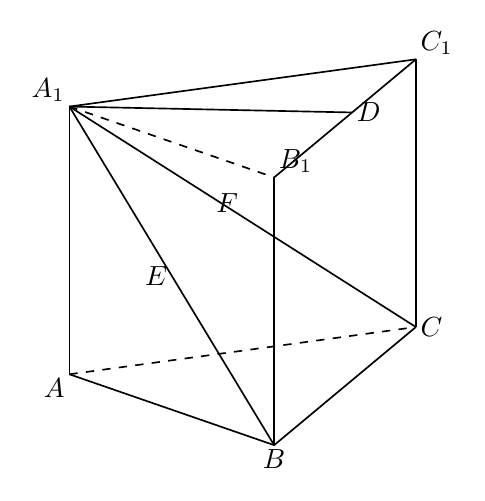
\begin{tikzpicture}[scale=1.0, semithick, every node/.style={inner sep=1.4pt}]
  \coordinate (A) at (0,0);
  \coordinate (A1) at (0,3.4);
  \coordinate (B) at (2.6,-0.9);
  \coordinate (B1) at (2.6,2.5);
  \coordinate (C) at (4.4,0.6);
  \coordinate (C1) at (4.4,4.0);
  \coordinate (D) at (3.59,3.325);
  \coordinate (E) at (1.3,1.25);
  \coordinate (F) at (2.2,2.0);

  % 前面与可见棱
  \draw (A) -- (B) -- (C);
  \draw (A) -- (A1);
  \draw (B) -- (B1);
  \draw (C) -- (C1);
  \draw (A1) -- (C1);
  \draw (B1) -- (C1);
  % 面内连线
  \draw (A1) -- (B);
  \draw (A1) -- (C);
  \draw (A1) -- (D);

  % 被遮挡的棱
  \draw[dashed] (A) -- (C);
  \draw[dashed] (A1) -- (B1);

  \node[above left] at (A1) {$A_1$};
  \node[above right] at (C1) {$C_1$};
  \node[above right] at (B1) {$B_1$};
  \node[right] at (D) {$D$};
  \node[left] at (E) {$E$};
  \node[above left] at (F) {$F$};
  \node[below left] at (A) {$A$};
  \node[right] at (C) {$C$};
  \node[below] at (B) {$B$};
\end{tikzpicture}
